%\documentclass[12pt,dvipsnames,t]{beamer}

\documentclass[handout,12pt]{beamer}
%\usepackage[overlay]{textpos}
%\usepackage{pgfpages}
%\pgfpagesuselayout{4 on 1}[letterpaper, border shrink = 5mm]

\newcommand{\toggle}[1]{%
\addtocounter{framenumber}{-1}#1 % Comment this out if extra slides should be omitted
}
\newcommand{\toggleafter}[1]{%
#1\addtocounter{framenumber}{-1} % Comment this out if extra slides should be omitted
}

% \usepackage[latin1]{inputenc}
% \usepackage[danish]{babel}
% \usepackage{booktabs,amsmath,amsbsy}
%\usepackage{pgfpages}
%\pgfpagesuselayout{4 on 1}[a4paper,border shrink=5mm,landscape]
\usepackage[latin1]{inputenc}
\usepackage[english]{babel}
%\usepackage{graphicx,rotating,booktabs,verbatim,amsmath,amsbsy}
\usepackage{graphicx,rotating,booktabs,verbatim,amsmath}
\usepackage{tikz}


\graphicspath{{C:/Users/janne.pitkaniemi/figures/}}
%\graphicspath{{C://Users/janne.pitkaniemi/SPE2017}}



\usetikzlibrary{positioning}
%\tikzstyle{line} = [draw, -latex']
\usetikzlibrary{shapes,arrows}
% Define block styles
\tikzstyle{block} = [rectangle, draw, 
    text width=5em, text centered, rounded corners, minimum height=3.5em]
\tikzstyle{line} = [draw, -latex']
\tikzstyle{block} = [draw,rectangle,thick,minimum height=2em,minimum width=2em]

\usepackage{listings}
\usepackage{xcolor}
\definecolor{light-gray}{gray}{0.95}
\definecolor{mygreen}{rgb}{0,0.6,0}
\definecolor{mygray}{rgb}{0.5,0.5,0.5}
\definecolor{mymauve}{rgb}{0.58,0,0.82}


\lstset{ %
  backgroundcolor=\color{light-gray},   % choose the background color; you must add %\usepackage{color} or \usepackage{xcolor}
  basicstyle=\footnotesize,        % the size of the fonts that are used for the code
  breakatwhitespace=false,         % sets if automatic breaks should only happen at whitespace
  breaklines=true,                 % sets automatic line breaking
  captionpos=b,                    % sets the caption-position to bottom
  commentstyle=\color{mygreen},    % comment style
  deletekeywords={...},            % if you want to delete keywords from the given language
  escapeinside={\%*}{*)},          % if you want to add LaTeX within your code
  extendedchars=true,              % lets you use non-ASCII characters; for 8-bits encodings only, does not work with UTF-8
  frame=single,                    % adds a frame around the code
  keepspaces=true,                 % keeps spaces in text, useful for keeping indentation of code (possibly needs columns=flexible)
  keywordstyle=\color{black},       % keyword style
  language=R,                 % the language of the code
  otherkeywords={*,...},            % if you want to add more keywords to the set
  numbers=left,                    % where to put the line-numbers; possible values are (none, left, right)
  numbersep=5pt,                   % how far the line-numbers are from the code
  numberstyle=\tiny\color{mygray}, % the style that is used for the line-numbers
  rulecolor=\color{black},         % if not set, the frame-color may be changed on line-breaks within not-black text (e.g. comments (green here))
  showspaces=false,                % show spaces everywhere adding particular underscores; it overrides 'showstringspaces'
  showstringspaces=false,          % underline spaces within strings only
  showtabs=false,                  % show tabs within strings adding particular underscores
  stepnumber=none,                    % the step between two line-numbers. If it's 1, each line will be numbered
  stringstyle=\color{mymauve},     % string literal style
  tabsize=2,                       % sets default tabsize to 2 spaces
  title=\lstname                   % show the filename of files included with \lstinputlisting; also try caption instead of title
}


\newcommand{\E}{\mathrm{E}}
\renewcommand{\P}{\mathrm{P}}
\newcommand{\Y}{\mathrm{\bf Y}}
\newcommand{\X}{\mathrm{\bf X}}
\newcommand{\I}{\mathrm{\bf I}}
\newcommand{\y}{\mathrm{\bf y}}
\newcommand{\h}{\mathrm{\bf h}}
\newcommand{\z}{\mathrm{\bf z}}
\newcommand{\x}{\mathrm{\bf x}}
\newcommand{\w}{\mathrm{\bf w}}
\newcommand{\e}{\mathrm{\bf e}}
\renewcommand{\v}{\mathrm{\bf v}}
\newcommand{\bnull}{\mathrm{\bf 0}}
\newcommand{\K}{\mathrm{\bf K}}
\newcommand{\Z}{\mathrm{\bf Z}}
\newcommand{\B}{\mathrm{\bf B}}
\newcommand{\eeta}{\mathrm{\bf \eta}}
\newcommand{\biota}{\mathrm{\bf \iota}}
\newcommand{\bepsilon}{\mathrm{\bf \epsilon}}
\newcommand{\bnu}{\mathrm{\bf \nu}}
\newcommand{\bbeta}{\mathrm{\bf \beta}}
\newcommand{\btheta}{\mathrm{\bf \theta}}
\newcommand{\bzeta}{\mathrm{\bf \zeta}}
\newcommand{\blambda}{\mathrm{\bf \lambda}}
\newcommand{\bLambda}{\mathrm{\bf \Lambda}}
\newcommand{\bGamma}{\mathrm{\bf \Gamma}}
\newcommand{\bPsi}{\mathrm{\bf \Psi}}
\newcommand{\bPi}{\mathrm{\bf \Pi}}


\definecolor{sinine}{rgb}{0.00,0.25,0.50}
\definecolor{dsinine}{rgb}{0.53,0.58,0.73}
\definecolor{punane}{rgb}{0.72,0.05,0.00}
\definecolor{roheline}{rgb}{0.2,0.4,0.1}
\definecolor{heleroheline}{rgb}{0.38,0.75,0.00}
\definecolor{dheleroheline}{rgb}{0.45,1.00,0.45}
\definecolor{droheline}{rgb}{0.8,0.9,0.6}


%----------------------------------------------------------------------
% The general look of things:

% Theme with navigation bar on the right; [width=0em] removes it
\mode<presentation>{\usetheme[width=0em]{Goettingen}}

% Omit the navigation symbols --- I have pg-up and pg-dn anyway
\setbeamertemplate{navigation symbols}{}

% Pagenumbering at the far right bottom corner
\setbeamertemplate{footline}{
  \usebeamercolor[fg]{frametitle}
  \hspace*{3ex}\currentlecture % This is for inserting title of the lecture
  \hfill \bf \insertframenumber / \inserttotalframenumber
  \rule[-2ex]{0pt}{5ex} \hspace*{3ex}}

% How visible should the uncovered items be? 0 corresponds to not at all.
\setbeamercovered{transparent=0}

% Get the fonts to look right in mathematics parts
\usefonttheme[onlymath]{serif}
%\input{beamer-math.tex} % A re-definition of all math
                        % commands (and some more) that
                        % makes them appear in serif font

% \input{useful}

% The heading font is a little too thin to my taste
\setbeamerfont{frametitle}{size=\large,series=\bfseries}

% Use pdf graphs
\DeclareGraphicsExtensions{.pdf,.jpg}

% End of setting up the formal layout of the slides

% Definition of a dummy command so that the above works and so that ALL
% redefinitions can be done by \renewcommand{\currentlecture}
\newcommand{\currentlecture}{}


% Tree drawing is from useful.tex which won;t load since it produces an error
% when trying to overwrite existing definitions

%
% Tree drawing
%
\newcommand{\tree}[3]{\setlength{\unitlength}{#1}\begin{picture}(0,0)
   \put(0,0){\line(3,2){1}}
   \put(0,0){\line(3,-2){1}}
   \put(0.81,0.54){\makebox(0,0)[br]{\footnotesize #2\ }}
   \put(0.81,-0.54){\makebox(0,0)[tr]{\footnotesize #3\ }}
\end{picture}}

\newcommand{\wtree}[3]{\setlength{\unitlength}{#1}\begin{picture}(0,0)
   \put(0,0){\line(1,1){1}}
   \put(0,0){\line(1,-1){1}}
   \put(0.8,0.8){\makebox(0,0)[br]{\footnotesize #2\ }}
   \put(0.8,-0.8){\makebox(0,0)[tr]{\footnotesize #3\ }}
\end{picture}}

\newcommand{\ntree}[3]{\setlength{\unitlength}{#1}\begin{picture}(0,0)
   \put(0,0){\line(2,1){1}}
   \put(0,0){\line(2,-1){1}}
   \put(0.8,0.4){\makebox(0,0)[br]{\footnotesize #2\ }}
   \put(0.8,-0.4){\makebox(0,0)[tr]{\footnotesize #3\ }}
\end{picture}}

\newcommand{\nutree}[3]{\begin{picture}(0,0)
   \put(0,0){\line(2,1){#1}}
   \put(0,0){\line(2,-1){#1}}
   \put(0.8,0.4){\makebox(0,0)[br]{#2\ }}
   \put(0.8,-0.4){\makebox(0,0)[tr]{#3\ }}
\end{picture}}

\newcommand{\bes}{\begin{eqnarray*}}
\newcommand{\ees}{\end{eqnarray*}}

% Commands to draw observation lines on follow-up diagrams
%
% Horizontal lines
%
\newcommand{\hfail}[1]{\begin{picture}(250,5)
      \put(0,0){\line(1,0){#1}}
      \put(#1,0){\circle*{5}}
   \end{picture}}

\newcommand{\hcens}[1]{\begin{picture}(250,5)
      \put(0,0){\line(1,0){#1}}
      \put(#1,0){\line(0,1){2.5}}
      \put(#1,0){\line(0,-1){2.5}}
   \end{picture}}

%----------------------------------------------------------------------
% It is more readable with a little extra space between paragraphs
\parskip 0.8ex

% \AtBeginSubsection[]
% {
%   \begin{frame}<beamer>
%     \frametitle{Outline}
%     \tableofcontents[currentsection,currentsubsection]
%   \end{frame}
% }
% \beamerdefaultoverlayspecification{<+->}

\title{Epidemiologic Data Analysis using R \\
Part 8:\\  Competing risk in time-to-event analysis}  % : \\ Analysis of Follow-up Studies}
% \Rlogo{height=1em} }

\author{Janne Pitk\"aniemi}

\institute{Finnish Cancer Registry, Finland,   
 \texttt{<janne.pitkaniemi@cancer.fi>} \\ }


\date{University of Tampere \\Faculty of Social Sciences \\ % University of Tampere/Postgraduate training,
Feb 26- Apr 9  2018}

\begin{document}

\maketitle


\begin{frame}
\frametitle{Points to be covered}

\begin{itemize}
\item[1.] 
Distribution concepts for times to event: \\ 
 survival, hazard and cumulative hazard,
 \medskip
 \item[2.] 
 Competing risks: event-specific cumulative incidences \& hazards.
 \medskip
\item[4.] Kaplan--Meier and Aalen--Johansen estimators.
 \medskip
 \item[5.] 
 Regression modelling of competing hazards:
 \medskip
 \item[6.]
 Packages \texttt{survival, mstate, cmprisk}.
\medskip
\item[7.] 
 Functions \texttt{Surv(), survfit(), plot.survfit(), coxph(), Cuminc()}.
\end{itemize}

Points not to be covered -- many!

\end{frame}


\begin{frame}
\frametitle{Survival time -- time to event}

Let $T$ be the \textbf{time} spent in a given \textbf{state} from its 
beginning till a certain \textit{endpoint} or \textit{outcome} \textbf{event} or \textit{transition}
 occurs, changing the state to another. \\
 (\texttt{lex.Cst - lex.dur - lex.Xst})

\bigskip
Examples of such times and outcome events:
\begin{itemize}
\item lifetime: birth $\rightarrow$ death,
\medskip
\item duration of marriage: wedding $\to$ divorce, 
\medskip
\item healthy exposure time: \\ start of exposure  
  $\rightarrow$ onset of disease,
  \medskip
\item clinical survival time: \\
 diagnosis of a disease  $\rightarrow$ death.
\end{itemize}


\end{frame}


%-----------------------------------

%----------------------------------------------------------------------
\begin{frame}
   \frametitle{Set-up of classical survival analysis} 

\begin{itemize}
\item
\textbf{Two-state model}: only one type of event changes the initial state.
\medskip
\item
Major applications: analysis of lifetimes
 since birth and of survival times since diagnosis of a disease 
 until death from any cause.
\end{itemize}

\setlength{\unitlength}{0.7pt}
% \begin{center}
\begin{picture}(400,80)(-40,70)
  \thicklines
  \put(  0, 80){\framebox(110,50){Alive}}
  \put(240, 80){\framebox(110,50){Dead}}
  \put(125,105){\vector(1, 0){100}}
  \put(170,110){\makebox(0,0)[b]{Transition}}
\end{picture}
% \end{center}

\begin{itemize}
\item
 \textbf{Censoring}: Death and final lifetime not observed
  for some subjects 
  %, as the follow-up terminates 
  due to emigration or closing the follow-up while they are still
 alive 
\end{itemize}

\end{frame}
  
% ------------------


\begin{frame}
\frametitle{Distribution concepts: survival function} 

Cumulative distribution function (CDF)
$F(t)$ and density function $f(t) =F'(t)$ of survival time $T$:
\[F(t) =  P( T \le t) = \int_0^t f(u) du \]
= \textbf{risk} or probability that the event occurs by $t$. 
% (probability of surviving at most up to $t$).

\bigskip
\textbf{Survival function} 
%\textcolor{red}{
\[ S(t) = 1- F(t) =  P( T  >  t) = \int_t^{\infty} f(u)du, \]
= probability of avoiding the event at least up to $t$
$\qquad\qquad{}$ (the event occurs
only after $t$).  

\end{frame}



\begin{frame}

\frametitle{Distribution concepts: hazard and cumulative function}

The \textbf{hazard rate} or \textbf{intensity} function $h(t)$
\begin{align*}
\lambda(t) & = \underset{\Delta \rightarrow 0}{\lim} 
 {P(t < T \le t+\Delta | T > t)}/{\Delta} \\
   & = \underset{\Delta \rightarrow 0}{\lim}\:
      \frac{P(t < T \le t+\Delta)}{P(T > t)}\: \frac{1}{\Delta}
     = \frac{f(t)}{S(t)}  
\end{align*}

%\begin{itemize}
%\item[$\approx$]  the conditional probability that
%the event occurs in a short
% interval $(t, t+\Delta]$, given that it does not
%occur before $t$, divided by interval length. 
%\end{itemize}

In other words, during a short interval
 \begin{center}
 risk of event $\approx$ hazard $\times$ interval length 
 \end{center}

The \textbf{cumulative hazard} (or integrated intensity):
\[
\Lambda(t) = \int_0^t \lambda(v)dv
\]

\end{frame}

%\begin{frame}
%Some examples: \\
%\includegraphics[width=23cm]{theordist}
%
%\end{frame}

%
%\begin{frame}
%\frametitle{Distribution: cumulative hazard etc.}
%
%The \textbf{cumulative hazard} (or integrated intensity):
%\[
%\Lambda(t) = \int_0^t \lambda(v)dv
%\]
%
%\bigskip
%Connections between the functions:
%\begin{eqnarray*}
%\lambda(t) & = & \frac{f(t)}{1-F(t)} =  -\frac{S'(t)}{S(t)} 
% = - \frac{d\ \log [ S(t)] }{d t} , \\
%\Lambda(t) & = & - \log [S(t)] , \\
%  S(t) & = & \exp\{ - \Lambda(t) \} 
%         = \exp\left\{ - \int_0^t \lambda(v)dv \right\}, \\
%  f(t) & = & \lambda(t)S(t) \\
%F(t) & = & 1 - \exp\{ - \Lambda(t) \} \\
%    &  = &  \int_0^t \lambda(v)S(v)dv  
%\end{eqnarray*}
%
%\end{frame}




%\begin{frame}
%\frametitle{Observed data on survival times}
%
%For individuals $i = 1, \dots, n$ let \\
%% $\quad B_i$ = time of entry to follow-up (often $B_i = 0$),  \\
%$\quad T_i$ = true time to outcome event,\\
%% $\quad C_i$ = variable for event 1, or 2, or censoring ,\\
%$\quad U_i$ = true time to censoring.\\
%\medskip
% Censoring is assumed \textbf{noninformative}, \textit{i.e.} \\ independent 
% from occurrence of events.
% 
% \pause\bigskip
%We observe 
%\begin{itemize}
%\item[ ]
%$y_i = \text{min}\{ T_i, U_i \}$, \textit{i.e.}
%the exit time, and
%\item[ ]
% $ \delta_{i} = 1_{ \{ T_i < U_i  \} }$, 
%  indicator (1/0) for the outcome event occurring first, before censoring. 
%\end{itemize}
%
%Censoring must properly be taken into account in the statistical analysis.
%
%% both in parametric likelihood-based inference and in non-parametric approaches.
%
%\end{frame}


\begin{frame}
\frametitle{Approaches for analysing survival time}

\begin{itemize}
\item 
\textbf{Parametric model} (like Weibull, gamma, etc.) on hazard rate $\lambda(t)$  
% fitted on survival times
% (like % exponential, %: $h(t) = \lambda$ (constant over time)
% Weibull, gamma, etc.) %: $h(t) = \kappa \lambda t^{\kappa-1}$
 %: $f(t) =  \lambda^\alpha 
%        t^{\alpha - 1} \exp( - \lambda t ) / \Gamma(\alpha)$
% lognormal, 
% $$ f(t) = \frac{1}{ y \sqrt{2\pi\sigma^2} }
%   \exp \left\{ - \frac{ [\log(t) - \mu]^2 }{2\sigma^2}  \right\}  $$
% log-logistic, generalized gamma, \textit{etc.}) \\ 
% $\to$ Likelihood:
%\begin{align*} L & = \prod_{i=1}^n \lambda(y_i)^{\delta_i} S(y_i) = 
%    \prod_{i=1}^n \lambda(y_i)^{\delta_i} \exp\{- \Lambda(y_i) \} \\
%   & =  \exp\left\{ \sum_{i=1}^n 
%     [ \delta_i \: \log \: \lambda(y_i) - \Lambda(y_i) ] 
%       \right\} 
%\end{align*}   
\item 
\textbf{Piecewise constant rate} model on $\lambda(t)$ \\ 
-- see Bendix's lecture on time-splitting. 
\medskip
\pause
\item 
\textbf{Non-parametric} methods, 
like \\ Kaplan--Meier (KM) % and Aalen--Johansen (AJ) 
estimator of survival curve $S(t)$ and Cox % and Fine \& Gray 
proportional hazards model on $\lambda(t)$.
% \\ -- The focus in this presentation.

\end{itemize}

\end{frame}
 

%\begin{frame}[fragile]
%
%\frametitle{R package \texttt{survival} }
%
%Tools for analysis with one outcome event.
%
%\begin{itemize}
%\item 
%\texttt{Surv(time, event) -> sobj} \\ 
%creates a \textbf{survival object} \texttt{sobj}, containing
% pairs $(y_i, \delta_i)$,
% \medskip
% \item
%\texttt{Surv(entry, exit, event) -> sobj2} \\
% creates a survival object from
%  \texttt{entry} and \texttt{exit} times, % \& event indicator,
%  \pause \medskip
%\item 
%\verb!survfit(sobj ~ x) -> sfo! \\
%creates a \textbf{survfit} object {\tt sfo}
%containing KM or other non-parametric estimates
%% from survival object  \texttt{sobj} 
%(also from a fitted Cox model), 
% \pause  \medskip
%\item 
%\texttt{plot(sfo)} \\
%% applied to \texttt{survfit} object \texttt{sfo}
% plot method for survival curves and related graphs, 
%\pause
%  \medskip
%\item 
%\verb|coxph(sobj ~ x1 + x2)| \\ 
%fits a Cox model
%% for the relative hazards to depend 
%with covariates \texttt{x1} and \texttt{x2}. 
%\pause
%    \medskip
%\item 
%\texttt{survreg()} -- parametric survival models.
%\end{itemize}   
%
%\end{frame}

\begin{frame}[fragile]
\frametitle{Ex. Survival of 338 oral cancer patients}

% Dataset \texttt{oralca.txt} describes the 
% Survival of patients with oral squamous cell
% carcinoma, treated at a tertiary level hospital. 
{Important variables}: 
\begin{itemize}
\item \texttt{time} = duration of patientship from \\ 
 diagnosis (\textbf{entry}) till death or censoring, 
\medskip
\item
\texttt{event} = indicator for the outcome and its \\
 observation at the end of follow-up (\textbf{exit}): \\
  0 = censoring,  \\
  1 = death from oral cancer, \\
  2 = death from some other cause.
\end{itemize}
% \texttt{Surv(time, event)} creates a \emph{survival} object.

\medskip
Special features:
\begin{itemize}
\item
   Several possible endpoints, \textit{i.e.} alternative causes of death, of which
   only one is realized.
   \medskip
\item
   Censoring -- incomplete observation of the survival time.   
\end{itemize}
\end{frame}



\begin{frame}[fragile]
\frametitle{Ex. Oral cancer data }

\begin{verbatim}
> head(orca)
     sex      age stage  time event
1   Male 65.42274  unkn 5.081     0
2 Female 83.08783   III 0.419     1
3   Male 52.59008    II 7.915     2
4   Male 77.08630     I 2.480     2
5   Male 80.33622    IV 2.500     1
6 Female 82.58132    IV 0.167     2
\end{verbatim}

\end{frame}

\begin{frame}[fragile]
\frametitle{Ex. Oral cancer data }

Analysis of overall motality

% \texttt{Surv(time, event)} creates a \emph{survival} object. Function % 
% \texttt{survfit} estimates the survival function non-parametrically.
\small
\begin{verbatim}
> orca$suob <- Surv(orca$time, 1*(orca$event > 0) )


> km1 <- survfit( suob ~ 1, data = orca)
> km1              #  brief  summary
records   n.max n.start  events  median 0.95LCL 0.95UCL 
 338.00  338.00  338.00  229.00    5.42    4.33    6.92 
 
> summary(km1)     #  detailed KM-estimate
\end{verbatim}
\scriptsize
\begin{verbatim}
   time n.risk n.event survival std.err lower 95% CI upper 95% CI
  0.085    338       2   0.9941 0.00417       0.9859        1.000
  0.162    336       2   0.9882 0.00588       0.9767        1.000
  0.167    334       4   0.9763 0.00827       0.9603        0.993
  0.170    330       2   0.9704 0.00922       0.9525        0.989
  0.246    328       1   0.9675 0.00965       0.9487        0.987
   ...  
\end{verbatim}

\normalsize

\end{frame}


\begin{frame}
\frametitle{Oral cancer: Kaplan-Meier estimates}

\begin{figure}
\centering
\includegraphics[width=1.0\textwidth]{orca_S-F_L} 
\end{figure}

\end{frame}

%\begin{frame}
%\frametitle{Estimated $F(t) = 1-S(t)$ on variable scales}
%\begin{itemize}
%\item
%KM curve of survival $S(t)$ is the most popular.
%\item 
%Informative  are also graphs for estimates of \\ 
%$\quad F(t) = 1- S(t)$, \textit{i.e.} CDF\\
%$\quad \Lambda(t) = -\log[ 1 - F(t)]$,  cumulative hazard, \\ 
%$\quad \log[ \Lambda(t) ]$, cloglog transform of CDF.
%\end{itemize}
%
%\includegraphics[width=\textwidth]{orcaKM2} 
%
%\end{frame}


%----------------------------------------------------------------------
\begin{frame}
   \frametitle{Competing risks model: causes of death}
   
\begin{itemize}
\item
Often the interest is focused on the risk or hazard of dying 
from one specific cause.
\medskip
\item
That cause may eventually not be realized, because
a \textbf{competing cause} of death hits first.

\bigskip

\begin{center}
\setlength{\unitlength}{0.65pt}
\begin{picture}(400,190)
  \thicklines
  \put(  0, 80){\framebox(120,50){Alive}}
  \put(230,130){\framebox(180,50){Dead from cancer}}
%  \put(170, 97){(Cause-specific hazards)}
  \put(230, 30){\framebox(180,50){Dead, other causes}}
  \put(135,125){\vector(3, 1){90}}
%  \put(295,155){\vector(0,-1){100}}
  \put(135, 85){\vector(3,-1){90}}
  \put(165,157){\makebox(0,0)[b]{$\lambda_1(t)$}}
  \put(165, 53){\makebox(0,0)[t]{$\lambda_2(t)$}}
% \put(285,105){\makebox(0,0)[t]{$\nu$}}
\end{picture}
\end{center}
\item
 Generalizes to several competing causes.
 \end{itemize}
% Illness-death model. Little boxes with arrows.\\
% (The mortality of lung cancer patients ($\nu$) not relevant here).
\end{frame}


%------------------
\begin{frame}
\frametitle{Competing events \& competing risks}

\begin{itemize}
\item \textbf{a competing risk} is an event that either
hinders the observation of the event of interest or modifies the
chance that this event occurs.
\item In those cases, the competing risk hinders the observation of the event of interest or modifies the chance that this event occurs.
\item  For example, when performing a
study with mortality on dialysis as the outcome of interest, a
patient may receive a kidney transplant. This transplant is a
competing risk because after the transplantation, this patient
is not on dialysis anymore and therefore no longer at risk of
dying while being on dialysis. In this case, the competing
event, i.e. receiving a kidney transplant, hinders the occurrence
of the event of interest.
\end{itemize}
\end{frame}

\begin{frame}
\frametitle{Research question is relevant for the method}

\begin{itemize}
\item There are two main methodological strems: \textbf{hazard and subdistribution approach} to estimation of parameters of interest.  
\item What kind of research question one aims to answer. In general,
there are two types of research questions which can be
answered with epidemiological studies. 
\item Aetiological research aims to investigate the causal relationship between risk factors or determinants and a given outcome. The effect is measures in HR.
\item Prognostic research aims to predict the probability of a given outcome at a given time for an individual patient.
\end{itemize}
\end{frame}

\begin{frame}
\frametitle{Competing events \& competing risks}

In many epidemiological and clinical contexts there are
competing events that may 
occur before the target event and remove the person from 
 the population at risk for the event, \textit{e.g.}

\begin{itemize}
\item \textit{target event}: occurrence of endometrial cancer,
 \textit{competing events}: hysterectomy or death.
\medskip
\item \textit{target event}: relapse of a disease \\
(ending the state of remission), \\
 \textit{competing event}: death while still in remission.
 
% \medskip
\item \textit{target event}: divorce, \\ 
 \textit{competing event}: death of either spouse.
 
\end{itemize}

\end{frame}

\begin{frame}
\frametitle{Event-specific quantities}

\textbf{Cumulative incidence function} (CIF) or \\
 \textbf{subdistribution function} for event $c$:
\[  F_c(t) = P(T \leq t \text{ and } C = c ), \quad c = 1,2,  \]
{subdensity function} $f_c(t) = dF_c(t)/dt$ 

\medskip
From these one can recover
\begin{itemize}
\item
$F(t) = \sum_{c} F_c(t)$, CDF of event-free survival time $T$, \textit{i.e.} 
cumulative risk of any event by $t$.
\medskip
\item
$S(t) = 1 - F(t)$, \textbf{event-free survival function}, \textit{i.e.} probability of avoiding all events by $t$
\end{itemize}
\end{frame}

\begin{frame}
\frametitle{Event-specific quantities (cont'd)}

%\begin{itemize}
%\item
\textbf{Event-} or \textbf{cause-specific hazard function}
\begin{align*}
 \lambda_c(t) & =  \underset{\Delta\to 0}{\lim} 
    \frac{P(t < T \le t+\Delta \text{ and } C = c \mid T > t)}{\Delta}  \\
        & =  \frac{f_c(t)}{1-F(t)}
% \underset{\Delta\to 0}{\lim} \frac{F_c(t+\Delta) - F_c(t)}{S(t)}/\Delta
\end{align*}
\begin{itemize}
\item[$\approx$] Risk of \textit{event} $c$ 
in a short interval $(t, t+ \Delta]$,  given 
\textit{avoidance of all events} up to $t$, 
per interval length.
\end{itemize}

\textbf{Event-} or \textbf{cause-specific cumulative hazard} 
 $$ \Lambda_c(t) = \int_0^t \lambda_c(v)dv $$ 

\end{frame}


\begin{frame}
\frametitle{Event-specific quantities (cont'd)}
\begin{itemize}
\item CIF = risk of event $c$ over risk period $[0,t]$ in the presence of competing risks, also obtained 
% $c$-specific hazard and overall survival:
$$ F_c(t) = \int_0^t \lambda_c(v) S(v) dv, \quad c = 1,2, $$
\item
Depends on the hazard of the competing event, too, 
via 
\begin{align*} 
S(t) & = \exp\left\{ - \int_0^t [\lambda_1(v) + \lambda_2(v)]dv 
 \right\} \\
 & = \exp\left\{ - \Lambda_1(t) \right\} \times        \exp\left\{ - \Lambda_2(t) \right\} .
\end{align*}
\end{itemize}
\textbf{Hazard of the subdistribution} \\
\begin{center}
  $\gamma_c(t) = {f_c(t)}/[1 - F_c(t)] $
\end{center}	
	% \qquad     [ \neq \lambda_c(t),\ \textbf{NB!}] \\
%  & = \underset{\Delta\to 0}{\lim} \
%    P \{ t < T \le t+\Delta \text{ and } C = c \mid \\
%  & \qquad\qquad   T > t \text{ or }  
%     ( T \leq t \text{ and }C \neq c) \}/{\Delta}  
\begin{itemize}
\item Is not the same as 
$\lambda_c(t) = f_c(t)/[1-F(t)]$,
\item Interpretation tricky!
\end{itemize}
\end{frame} 


\begin{frame}
\frametitle{Warning of ``net risk'' and ``cause-specific survival''}

\begin{itemize}                              
\item
The ``\textbf{\textit{net risk}}'' of outcome $c$ by time $t$, 
assuming hypothetical elimination of competing risks,
is often defined as
\begin{center}
$ F_c^*(t) = 1 - S_c^*(t) = 1- \exp\{ - \Lambda_c(t) \} $
% =1 - \exp\left\{ - \int_0^t h_c(v) dv \right\},  $$
\end{center}
\medskip
\item
In clinical survival studies, function 
$S_c^*(t)$ is often called ``\textbf{\textit{cause-specific survival}}'',
and estimated by KM, but treating competing deaths
as censorings.
\medskip
\item
Yet, these *-functions, $ F_c^*(t)$ and $S_c^*(t)$, lack proper probability interpretation when
 competing risks exist.
\medskip
\item
Hence, their use and naive KM estimation should be viewed critically
(Andersen \& Keiding, \textit{Stat Med}, 2012)
\end{itemize}
\end{frame}


%----------------------------------------------------------------------
\begin{frame}
   \frametitle{Example: Risk of lung cancer by age $a$?}
% \vspace*{-1em}
% \[
% \ptxt{Lung cancer before age 75} \ne 1-\e^{-\Lambda(75)}
% \]
% does not take the possibility of death prior to lung cancer into
% account.

\begin{itemize}
\item 
 Empirical \textbf{cumulative rate} 
CR$(a) = \sum_{k < a} I_k \Delta_k$, i.e.
 ageband-width ($\Delta_k$) weighted 
 sum of empirical 
 age-specific incidence rates $I_k$
 up to a given age $a$ \\
 = estimate of cumulative hazard $\Lambda_c(a)$.
 \medskip
 \item 
 Nordcan \& Globocan give 
``\textbf{\textit{cumulative risk}}'' by 75 y of age, computed from 
$1 - \exp\{-\text{CR}(75)\}$, as an estimate  of the probability of 
getting cancer before age $75$ y, 
assuming that death were avoided by that age. This is based on 
deriving ``net risk'' from cumulative hazard:
\begin{center} 
$ F_c^*(a) = 1 - \exp\{ - \Lambda_c(a) \}. $
\end{center}
\medskip
\item
Yet, cancer occurs in a mortal population.
\medskip
\item
As such CR$({75})$ is a sound age-standardized summary 
 measure for comparing cancer incidence across populations 
 based on a neutral standard population.
\end{itemize}

\end{frame}
 
 
%----------------------------------------------------------------------
 
%----------------------------------------------------------------------
\begin{frame}
\frametitle{Example. Male lung cancer in Denmark}

Event-specific hazards $\lambda_c(a)$ by age estimated by age-spec. rates of death and lung ca., resp.

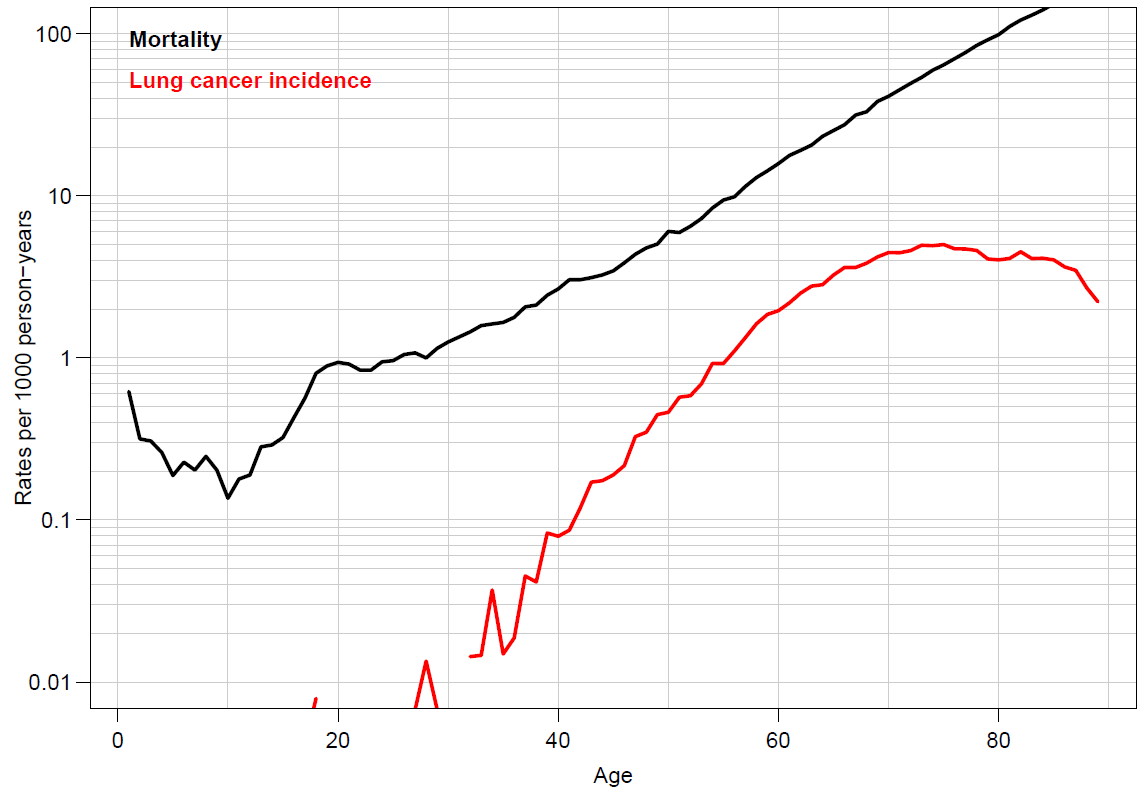
\includegraphics[height=6.5cm]{lung-ca-rates}
\end{frame}
  
%----------------------------------------------------------------------

%----------------------------------------------------------------------
\begin{frame}
\frametitle{Cumulative incidence of lung cancer by age}

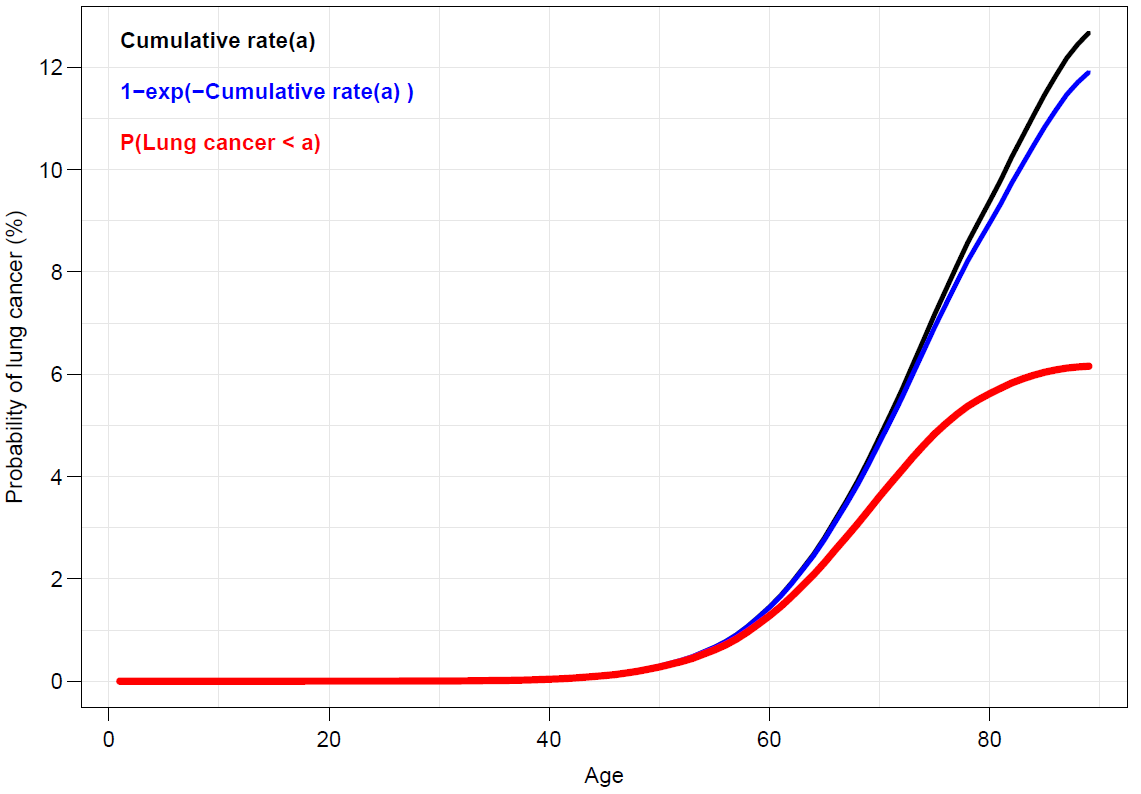
\includegraphics[height=6.5cm]{lung-ca-prob}

Both \text{CR} and $1 - \exp(- \text{CR})$ tend to \\
 overestimate the real cumulative incidence CI after 60 y.
\end{frame}
  
%----------------------------------------------------------------------
\begin{comment}
\begin{frame} \frametitle{Assumptions}
\begin{itemize}
\item
  The assumption behind the calculation and the statement ``6\% of
  Danish males will get lung cancer'' is that the lung cancer rates
  and the mortality rates in the file applies to a cohort of men. 
\item
  But they are cross-sectional rates, so the assumption is one of steady
  state of\\ 1: mortality rates (which is dubious)\\ and\\ 2: lung cancer
  incidence rates (which is appealing).
\item
  However the machinery can be applied to any set of rates for
  competing risks, regardless of how they were estimated.
\end{itemize}  
\end{frame}
 
\end{comment}  
%----------  



% \end{document}
%
%\begin{frame}
%\frametitle{Analysis with competing events}
%
%Let $U_i$ = censoring time, 
%% $\quad B_i$ = time of entry to follow-up (often $B_i = 0$),  \\
%$T_i$ = time to first event, and \\
%$C_i$ = variable for event 1 or 2. %, $i=1, \dots, n$. \\
%We observe 
%\begin{itemize}
%\item $y_i = \text{min}\{ T_i, U_i \}$, \textit{i.e.}
%the exit time, and
%\item
% $ \delta_{ic} = 1_{ \{ T_i < U_i \ \& \ C_i = c\} }$, 
%  indicator (1/0) for \\ 
%  event $c$ being first observed, $c=1,2$. 
%\end{itemize}
%Likelihood factorizes into event-specific parts:
%\begin{align*}
% L & = \prod_{i=1}^n \lambda_1(y_i)^{\delta_{i1}} 
% \lambda_2(y_i)^{\delta_{i2}} S(y_i) = L_1 L_2 \\
%   & = \prod_{i=1}^n \lambda_1(y_i)^{\delta_{i1}} 
%	 \exp\{ - \Lambda_1 (y_i) \} \times \prod_{i=1}^n
% \lambda_2(y_i)^{\delta_{i2}}  \exp\{ - \Lambda_2(y_i) \}
%% \\
%%   & = \exp\left\{ \sum_{c=1}^2  \sum_{i=1}^n 
%%   [ {\delta_{ic}}\: \log\: \lambda_c(y_i) - \Lambda_c(y_i) ] \right\}
%\end{align*}
%$\Rightarrow$ If $\lambda_1(y_i)$ and $\lambda_2(y_i)$ have no common parameters,
%% event-specific hazards 
%they may be fitted separately treating competing events
%as censorings. \\ -- Still, avoid estimating ``net risks'' from 
%$F_c^* = 1 - \exp(-\Lambda_c)$! 
%
%\end{frame}

\begin{frame}

\frametitle{Non-parametric estimation % $\widetilde{F}_c(t)$ 
of CIF} 

\begin{itemize}
\item
Let $t_1 < t_2 < \dots < t_K$ be the $K$ distinct 
time points at which any outcome event was observed, \\ Let also
 $\widetilde{S}(t)$ be KM estimator for overall $S(t)$. 
\medskip
\item
\textbf{Aalen-Johansen estimator} (AJ) for the cumulative incidence function $F(t)$
is obtained as
$$ \widetilde{F}_c(t) 
   = \sum_{t_k \leq t} \frac{D_{kc}}{n_k} \times \widetilde{S}(t_{k-1}),
   \quad\text{where}
$$
$n_k$ = size of the risk set at $t_k$ $(k=1, \dots, K)$,
\\
$D_{kc}$ = no. of cases of event $c$ observed  at $t_k$.
\medskip
\item
% \medskip
Naive KM estimator $\widetilde{F}^*_c(t)$ of ``net survival'' treats  
competing events occuring first as censorings:  
$$  \widetilde{F}^*_c(t) = 1 - \widetilde{S}^*_c(t)
  = 1 - \prod_{t_k \leq t} \frac{n_k - D_{kc}}{n_k} $$
\end{itemize}

\end{frame}



\begin{frame}

\frametitle{R tools for competing risks analysis}

Package \texttt{mstate}
\begin{itemize}
% \item Covers even more general multi-state set-ups.
%  \pause
%  \medskip
\item \texttt{Cuminc(time, status, ...)}:  \\
 AJ-estimates (and SEs) for each event type 
 % from observed follow-up times and events
  (\texttt{status}, value 0 indicating censoring)
\end{itemize}
Package \texttt{cmprsk}
\begin{itemize}
\item \texttt{cuminc(ftime, fstatus, ...)} 
  computes CIF-estimates,  % in \texttt{mstate},
   \texttt{plot.cuminc()} plots them. 
  \medskip
\item \texttt{crr()}
 fits Fine--Gray models for 
the hazard $\gamma_c(t)$ of the subdistribution
\end{itemize}   
Package \texttt{Epi} -- \texttt{Lexis} tools for multistate analyses
\begin{itemize}
\item  will be advertised by Bendix!
\end{itemize}

\end{frame}

\begin{frame}[fragile]
\frametitle{Ex. Survival from oral cancer}

\begin{itemize}
\item
Creating a {\tt Lexis} object with two outcome events and \\ 
obtaining a summary of transitions
\end{itemize}
\small
\begin{verbatim}
> orca.lex <- Lexis(exit = list(stime = time), 
           exit.status = factor(event, 
    labels = c("Alive", "Oral ca. death", "Other death") ),
                  data = orca)

> summary(orca.lex)  
Transitions:
     To
From    Alive Oral ca. Other  Records:  Events: Risk time:  Persons:
  Alive   109      122   107       338      229    1913.67       338
\end{verbatim}
\normalsize

\end{frame}

\begin{frame}[fragile]
\frametitle{Box diagram for transitions}

Interactive use of function {\tt boxes()}.
\small
\begin{verbatim}
> boxes(orca.lex)
\end{verbatim}
\begin{center}
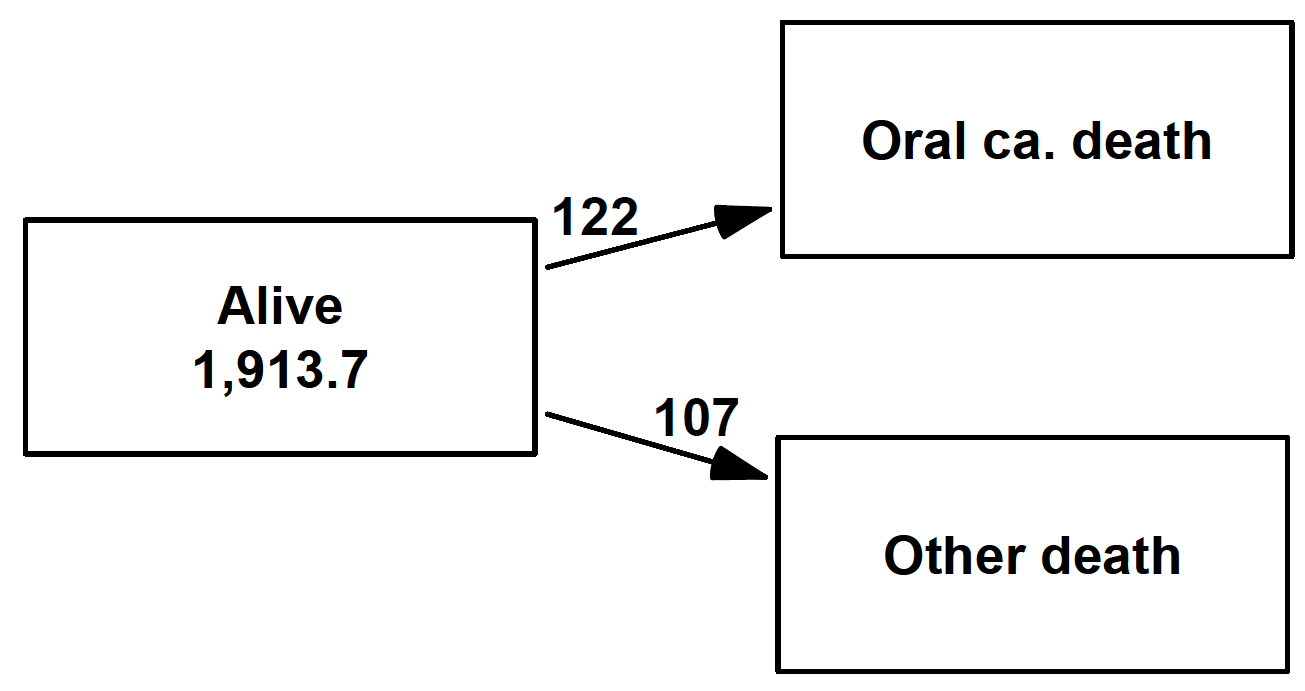
\includegraphics[height=6cm]{orca-boxes}
\end{center}
\normalsize

\end{frame}

\begin{frame}[fragile]
\frametitle{Ex. Survival from oral cancer}
\begin{itemize}
\item
AJ-estimates of CIFs (solid) for both causes.
\item
Naive KM-estimates of CIF (dashed) $>$ AJ-estimates 
\item
CIF curves may also be stacked (right).  
\end{itemize}
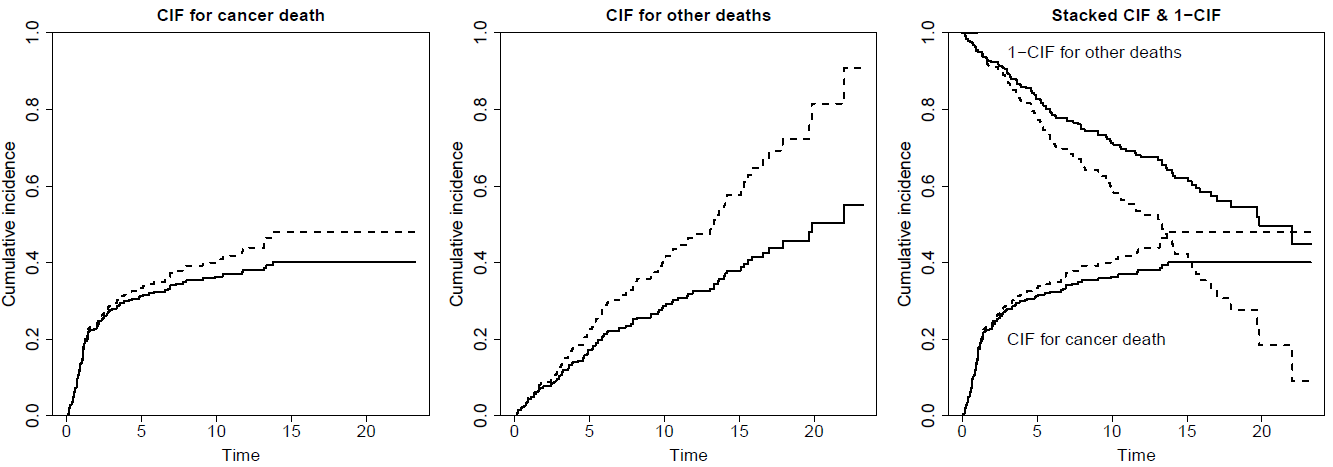
\includegraphics[width=\textwidth]{orcaCI1}

\textbf{NB.} The sum of the naive KM-estimates of CIF exceeds 100\% at 13 years! 
\end{frame}

\begin{frame}[fragile]
\frametitle{Ex. CIFs by cause in men and women}

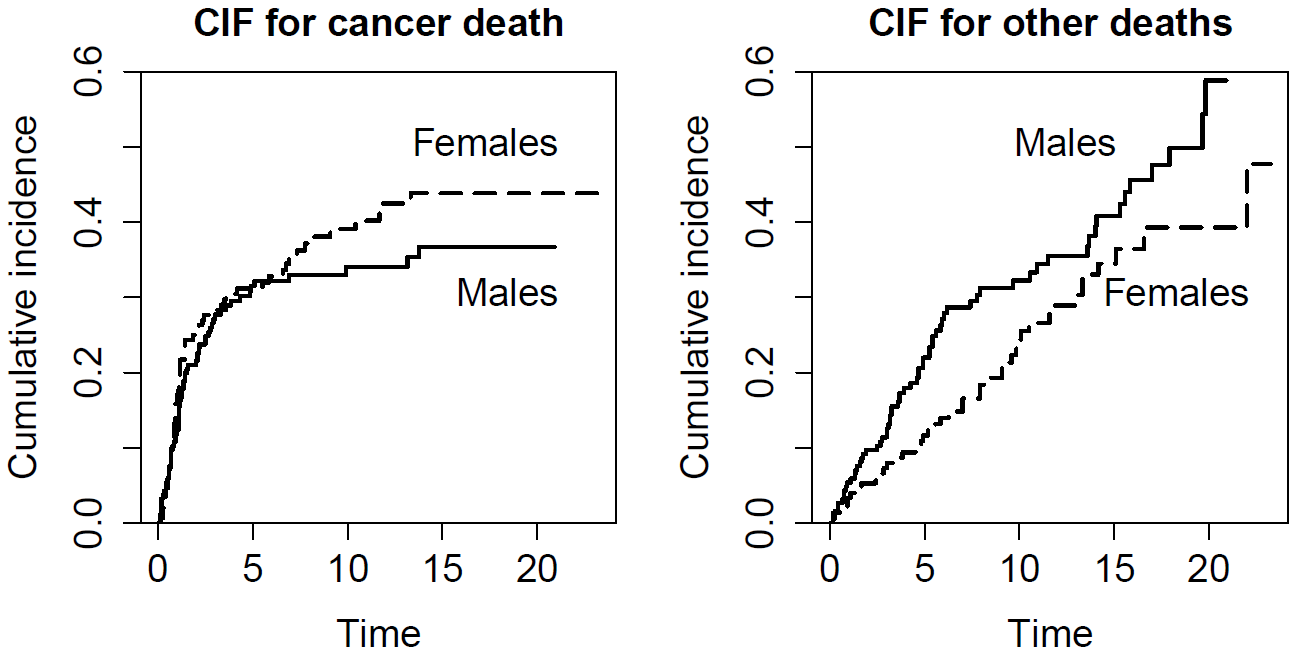
\includegraphics[width=\textwidth]{orcaCI2}

CIF for cancer higher in women (chance?) but for other causes
higher in men (no surprise).

\end{frame}

%\begin{frame}
%
%\frametitle{Regression models for time-to-event data}
%
%Consider only one outcome \& no competing events
% \begin{itemize} 
% \item
%Subject $i$ $(i=1, \dots, n)$ has an own vector $x_i$ that contains
% values $(x_{i1}, \dots, x_{ip})$ of a set of $p$ 
%continuous and/or binary covariate terms.
%\pause
%\medskip
%\item
% In the spirit of generalized linear models we let 
%  $\beta = (\beta_1, \dots, \beta_p)$ be regression coefficients
%  and build  a \textbf{linear predictor} 
% $$ \eta_i =
%x_i^{\small\text{T}} \beta =  \beta_1 x_{i1} + \dots + \beta_p x_{ip} $$ 
%\item
%Specification of outcome variable? \\
% Distribution (family)? Expectation? Link?  
%\end{itemize} 
%\end{frame}
%
%
%
%\begin{frame}
%\frametitle{Regression models (cont'd)}
%  
%Survival regression models can be defined \textit{e.g.} for 
%\begin{itemize}
%\item[(a)] survival times directly 
%$$ \log(T_i) = \eta_i + \epsilon_i, \quad\text{s.t. } 
%\epsilon_i \sim F_0(t; \alpha)$$ 
%where $F_0(t; \alpha)$ is some baseline model, 
%\medskip
%\pause
%\item[(b)] hazards, multiplicatively: $$ 
%\lambda_i(t) = \lambda_0(t; \alpha) r(\eta_i), \quad\text{where}$$
%$\lambda_0(t; \alpha)$ = baseline hazard and \\
%$r(\eta_i)$ = relative rate function, typically $\exp(\eta_i)$
%\medskip
%\pause
%\item[(c)] hazards, additively: 
%$$ \lambda_i(t) = \lambda_0(t; \alpha) + \eta_i. $$
%\end{itemize}
%\end{frame}
%
%
%%\end{frame}
%
%
%\begin{frame}
%\frametitle{Relative hazards model or Cox model}
%
%In model (b), the baseline hazard $\lambda_0(t,\alpha)$ may be given a parametric form (\textit{e.g.} Weibull) or
%a piecewise constant rate (exponential) structure.
%
%\bigskip
%Often a parameter-free form $\lambda_0(t)$ is assumed. Then
%\[
%  \lambda_i(t) = \lambda_0(t) \exp(\eta_1),
%\]
%specifies the \textbf{Cox model} or the \textbf{semiparametric proportional hazards model}.
%
%\bigskip
%$\eta_i = \beta_1 x_{i1} + \dots + \beta_p x_{ip}$ not depending on time.  
%
%\bigskip
%Generalizations: \textbf{time-dependent} \\ covariates $x_{ij}(t)$, and/or 
%effects $\beta_j(t)$.
%
%% For exponential model, $\lambda_0(t) = \lambda_0$.
%
%% Piecewise exponential model $\to$ constant baseline
%% hazard in successive intervals:   
%% \[ 
%% \lambda_0(t) = \lambda_{0k}, \mbox{ for } 
%% a_{k-1}} < t \leq a_k, \quad k = 1, 2, \dots, K 
%% \]
%
%\end{frame}
%
%
%
%\begin{frame}
%\frametitle{PH model: interpretation of parameters}
%
%Present the model explicitly in terms of $x$'s and $\beta$'s.
%\[
%\lambda_i(t) = \lambda_0(t)  \exp({\beta_1 x_{i1} + \dots +
%\beta_p x_{ip}})
%\]
%Consider two individuals, $i$ and $i'$, having the same values of all
%other covariates except the $j^{\text{th}}$ one.
%
%\bigskip
%The ratio of hazards is constant:
%$$  \frac{\lambda_i(t)}{\lambda_{i'}(t)} = \frac{\exp( \eta_{i}) }{\exp(\eta_{i'})}
%= \exp \{ \beta_j(x_{ij}-x_{i'j}) \} . $$
%Thus $e^{\beta_j} = \text{HR}_j$ = \textbf{hazard ratio} or relative rate
% associated with
% a unit change in covariate $X_j$.
%
%\end{frame}
%
%\begin{frame}
%\frametitle{Fitting the Cox PH model}
%
%% Baseline $\lambda_0(t)$: a lot of nuisance parameters. 
%% Their inclusion used to make likelihood computations infeasible.
%
%\underline{Solution 1}: Cox's \textbf{partial likelihood}
% $L^P = \prod_k L^P_k $, ignores $\lambda_0(t_k)$ when estimating
%  $\beta$, using only the ordering of
%the observed  event times $t_k$: 
%\begin{align*}
% L^P_k & =   P(\text{the event occurs for }i_k\ | 
%               \text{ an event at }t_k)  \\
%  & = \exp(\eta_{i_k} ) /  \sum_{i\in R(t_k)} \exp(\eta_i), 
%  \quad\text{ where}
%\end{align*}  
%% $\eta_{i_k}$ belongs to the very subject
% $i_k$ = the subject encountering the event at $t_k$, \\
% $R(t_k)$ = {\bf risk set} = subjects at risk at $t_k$. 
% 
%\bigskip
%\underline{Solution 2}: Piecewise constant rate model with dense division of the time axis, and fitting by Poisson regression using \texttt{glm()} 
%(profile likelihood!).
%\end{frame}
%
%\begin{comment}
%\begin{frame}
%\frametitle{Fitting the Cox PH model (cont'd)}
%
%The $\beta$ parameters  are estimated by maximising 
%$\log (L^P)$. The partial information matrix $J^P(\beta)$ with
%$$ [J^P(\beta)]_{jl} = - \frac{ \partial^2 \log (L^P) }
%   {\partial \beta_j \partial \beta_l}, \quad j, l = 1, \dots, p $$
% is used in statistical inference, like the observed
% information matrix $J$ in ordinary likelihood models.  
%
% The baseline cumulative hazard $H_0(t)$ and survival
%$S_0(t)$ is then estimated by Aalen-Breslow estimator.
%
%{\bf NB.} This partial likelihood is equal to the
%\textbf{profile likelihood} of $\beta$ parameters in a Poisson regression model
%with ``dense" subdivision of time. 
%% when the hazard is assumed constant between consecutive
%% (distinct) observed failure times $t_k$, $k=1, \dots, D$.
%
%\end{frame}
%
%\end{comment}
%\begin{frame}[fragile]
%\frametitle{Ex. Total mortality of oral ca. patients}
%
%Fitting Cox models with sex and sex + age.
%\small
%\begin{verbatim}
%> cm0 <- coxph( suob ~ sex, data = orca)
%> summary( cm0)
%        coef exp(coef) se(coef)    z Pr(>|z|)
%sexMale 0.126     1.134    0.134 0.94     0.35
%        exp(coef) exp(-coef) lower .95 upper .95
%sexMale      1.13      0.882     0.872      1.47
%
%> cm1 <- coxph( suob ~ sex + age, data = orca)
%> summary(cm1)
%        exp(coef) exp(-coef) lower .95 upper .95
%sexMale      1.49      0.669      1.14      1.96
%age          1.04      0.960      1.03      1.05
%\end{verbatim}
%\normalsize
%The M/F contrast visible only after age-adjustment.
%\end{frame}
%
%\begin{frame}[fragile]
%\frametitle{Predictions from the Cox model}
%\begin{itemize}
%\item
%Individual survival \textit{times} cannot be predicted
%but ind'l survival \emph{curves} can.
%PH model implies:
%\[
%S_i(t) = [S_0(t) ]^{\exp(\beta_1 x_{i1} +\ldots+\beta_p x_{ip})}
%\]
%\item
%Having  estimated $\beta$ by partial likelihood, 
%the baseline $S_0(t)$ is estimated by Breslow method 
%\item 
%\medskip
% From these, a survival curve for an individual
%with given covariate values is predicted.
%\item
%\medskip
%In R: 
%\texttt{pred <- survfit(mod, newdata=...)} 
%and \texttt{plot(pred)}, where \texttt{mod} is the fitted
%\texttt{coxph} object, 
%and \texttt{newdata}  
%specifies the covariate values.
%\end{itemize}
%\end{frame}
%
%
%\begin{frame}
%\frametitle{Proportionalilty of hazards?}
%\begin{itemize}
%% \item
%%\emph{How to check this key assumption?}
%\item
%Consider two groups $g$ and $h$ defined by one categorical covariate, and let $\rho > 0$. 
%
%\medskip
%If $\lambda_g(t) = \rho \lambda_h(t)$  then 
%$\Lambda_g (t) = \rho \Lambda_h(t)$ and
%$$ \log\: \Lambda_g  (t)  = \log (\rho) + \log\: \Lambda_h (t), $$
%thus log-cumulative hazards should be parallel!
%\bigskip
%\item[$\Rightarrow$] 
%\textit{Plot the estimated log-cumulative hazards and see
%whether they are sufficiently parallel}.
%\bigskip
%\item
%% Recall that $\log\: \Lambda (t)  = \log[- \log \: S(t)]$. Hence,
%\texttt{plot(coxobj, ..., fun = 'cloglog')}
%% meaning \textbf{complementary log-log} transform of $S(t)$,
%% produces the desired graph.
%\medskip
%\item
%Testing the proportionality assumptions: \texttt{cox.zph(coxobj)}.
%\end{itemize}
%\end{frame}
%
%\begin{frame} 
%\frametitle{Ex. Mortality of oral cancer patients}
%
%Complementary log-log plots of total mortality by 
%\begin{itemize}
%\item
%age: 15-54 y (dash),
%55-74 y (solid), \\ 75+ y (longdash),
%\item sex: females (solid) and males (longdash).
%\end{itemize}
%
%\includegraphics[width=\textwidth]{orcaKM3}
%
%\end{frame}
%
%
%\begin{comment}
%
%
%
%\begin{frame}[fragile]
%
%\frametitle{Testing proportionality of hazards}
%
%With $>1$ covariates,  \texttt{cox.zph()} tests the assumption by checking,
%whether the corresponding parameters (\& hazard ratios)
%may vary in time.
%\small
%\begin{verbatim}
%> cox.zph(cm1)
%             rho   chisq     p
%sexMale -0.00459 0.00469 0.945
%age      0.06679 1.06403 0.302
%GLOBAL        NA 1.17663 0.555
%\end{verbatim}
%\normalsize
%No evidence against proportionality. 
%
%\end{frame}
%
%\end{comment}
%
%\begin{frame}[fragile]
%\frametitle{Non-proportionality w.r.t. one covariate?}
%
%If the covariate is not an exposure of interest, but needs to be adjusted for $\rightarrow$ fit a \textbf{stratified} model.
%
%Allows different baseline hazards, but same relative 
%effects of other covariates in each strata.
%
%\small
%\begin{verbatim}
%> cm2 <- coxph( suob ~ sex + strata(age3), data = orca)
%> summary(cm2) 
%
%        exp(coef) exp(-coef) lower .95 upper .95
%sexMale      1.35       0.74      1.03      1.77
%\end{verbatim}
%\normalsize
%
%If the covariate \textit{is} a factor of interest, one may consider transformations of it -- or a completely
%different model: a \textit{non-proportional} one!
%\end{frame}
%
%\begin{frame}
%\frametitle{Modelling with competing risks}
%
%% When more than one outcome are operating,
%% one may consider the 
%Main options, providing answers to different questions.
%
%\begin{itemize}
%\item[(a)]
%  Cox model for event-specific hazards $\lambda_c(t) = f_c(t)/[1-F(t)]$, when \textit{e.g.} the interest is in the biological effect of the prognostic factors on the fatality of the very disease that often leads to the relevant outcome.  
%  \bigskip 
%\item[(b)]
% \textbf{Fine--Gray model} for the hazard  of the subdistribution $\gamma_c(t) = f_c(t)/[1-F_c(t)]$ 
%  when we want to assess the impact of the factors on the overall cumulative incidence of event $c$.  \\
%  -- Function \texttt{crr()} in package \texttt{cmprsk}. 
%\end{itemize}
%
%\end{frame}

\end{document}
